\chapter{Θεωρητικό Υπόβαθρο}

\section{Βάσεις δεδομένων}

Με τον όρο βάση δεδομένων εννοούμε μία συλλογή από οργανωμένα δεδομένα, τα οποία μπορούν διαχειριστούν με εύκολο τρόπο. Ένα σύστημα διαχείρισης βάσεων δεδομένων 
είναι ένα λογισμικό που αλληλεπιδρά με τον χρήστη και άλλες εφαρμογές, με σκοπό τον ορισμό, την πρόσβαση, τη διαχείριση και τις επερωτήσεις στα δεδομένα που είναι 
αποθηκευμένα στη βάση δεδομένων. Οι βάσεις δεδομένων χρησιμοποιούνται ευρέως σε πολλές υπηρεσίες που αφορούν διάφορους τομείς της ανθρώπινης δραστηριότητας, όπως 
υπηρεσίες που προσφέρονται από τράπεζες, πανεπιστήμια και τηλεπικοινωνιακούς φορείς.

\subsection{Σχεσιακή βάση δεδομένων}

Ο όρος σχεσιακή βάση δεδομένων χρησιμοποιείται για να περιγράψει μία βάση δεδομένων που οργανώνει τα δεδομένα της με γνώμονα το σχεσιακό μοντέλο δεδομένων. Σύμφωνα 
με το μοντέλο αυτό, τα δεδομένα οργανώνονται σε πίνακες από γραμμές και στήλες, με κάθε γραμμή να περιέχει ένα μοναδικό κλειδί. Ο πίνακας αντιπροσωπεύει μία οντότητα, 
κάθε γραμμή αντιστοιχεί σε μία εφαρμογή της οντότητας και οι στήλες αποτελούν χαρακτηριστικά της οντότητας. Ανάμεσα στους διάφορους πίνακες της βάσης μπορεί να υπάρχουν 
σχέσεις από 'έναν σε έναν', από 'έναν σε πολλούς' ή και από 'πολλούς σε πολλούς', όπως χαρακτηριστικά ονομάζονται. Πιο συγκεκριμένα, η σχέση είναι ένα σύνολο από 
εγγραφές-γραμμές πινάκων που έχουν κοινά γνωρίσματα-στήλες. Άλλοι όροι που συναντά κανείς σε μία σχεσιακή βάση δεδομένων είναι το πρωτεύον κλειδί, το οποίο είναι ένα 
μοναδικό αναγνωριστικό μίας εγγραφής σε έναν πίνακα. Όταν ένα πρωτεύον κλειδί, είναι κοινό και για έναν άλλον πίνακα, τότε γίνεται εξωτερικό κλειδί στον πίνακα αυτό. Τέλος, 
το ευρετήριο σε ένα γνώρισμα μίας σχέσης είναι μία δομή αναζήτησης η οποία παρέχει γρηγορότερη πρόσβαση στα δεδομένα.

\subsection{Σύνολο ιδιοτήτων ACID}

Ένα σύστημα διαχείρισης βάσεων δεδομένων πρέπει να είναι συμβατό με το σύνολο ιδιοτήτων ACID, έτσι ώστε η λειτουργία της βάσης να θεωρείται έγκυρη και αποτελεσματική. 
Πρόκειται για τέσσερις βασικές αρχές που εξασφαλίζουν την αξιόπιστη ολοκλήρωση των δοσοληψιών σε μία βάση δεδομένων. Οι αρχές αυτές είναι η ατομικότητα, η συνέπεια, 
η απομόνωση και η μονιμότητα. Πιο αναλυτικά, η ατομικότητα απαιτεί η τροποποίηση, που θα γίνει στη βάση δεδομένων, να πραγματοποιηθεί είτε ολόκληρη είτε καθόλου. 
Έτσι, αν ένα μέρος της δοσοληψίας αποτύχει, θα πρέπει να αποτύχει και ολόκληρη η δοσοληψία. Η συνέπεια διασφαλίζει ότι η βάση δεδομένων θα βρίσκεται πάντα σε συνεπή 
κατάσταση. Η απομόνωση προϋποθέτει ότι οι δοσοληψίες δε μπορούν να έχουν πρόσβαση σε δεδομένα της βάσης τα οποία τροποποιούνται εκείνη τη στιγμή από κάποια άλλη δοσολοψία. 
Τέλος, η μονιμότητα εγγυάται στον χρήστη ότι τα αποτελέσματα μίας ολοκληρωμένης δοσοληψίας θα παραμείνουν στη βάση δεδομένων ακόμη και σε περίπτωση σφάλματος ή 
διακοπής λειτουργίας του συστήματος διαχείρισης της βάσης δεδομένων. 


\section{PostgreSQL}

Η PostgreSQL είναι μία αντικειμενοστρεφής-σχεσιακή βάση δεδομένων ανοιχτού κώδικα. Παρέχει πλήρη υποστήριξη για εξωτερικά κλειδιά, συνενώσεις, όψεις και πληθώρα 
τύπων δεδομένων. Μπορεί να εγκατασταθεί στα περισσότερα δημοφιλή λειτουργικά συστήματα, όπως Unix και Windows. Επίσης, διαθέτει περιβάλλον ανάπτυξης κώδικα σε γλώσσες 
προγραμματισμού, όπως C/C++, Java, Perl, Python, Ruby. Μπορεί να διαχειριστεί εύκολα μεγάλους αριθμούς ταυτόχρονων χρηστών καθώς και μεγάλο όγκο δεδομένων. Ενδεικτικά, 
το μέγιστο μέγεθος πίνακα είναι 32ΤΒ, εγγραφής είναι 1.6ΤΒ, πεδίου 1GB, ενώ τα μέγιστα μεγέθη βάσης, πλήθους εγγραφών και ευρετηρίων σε κάθε πίνακα είναι απεριόριστα. 
Επιπλέον, δίνει τη δυνατότητα στον χρήστη να δημιουργήσει νέους τύπους δεδομένων αλλά και να ορίσει νέες συναρτήσεις. Επιπρόσθετα, διαχωρίζει τα δικαιώματα πρόσβασης στα 
σχήματα της βάσης με τη λογική των ρόλων. Κάθε ρόλος αντιπροσωπεύει έναν μεμονωμένο ή μία ομάδα χρηστών που έχουν με συγκεκριμένα δικαιώματα πρόσβασης στο κάθε σχήμα 
της βάσης. Τέλος, η PostgreSQL υποστηρίζει διάφορες επεκτάσεις που προσδίδουν επιπλέον δυνατότητες στη λειτουργία και χρήση της.

\subsection{PostGIS}

Το PostGIS είναι μία επέκταση της PostgreSQL, η οποία παρέχει υποστήριξη για γεωγραφικά αντικείμενα στη βάση. Στην ουσία δίνει τη δυνατότητα στη βάση να αποθηκεύει 
και να διαχειρίζεται χωρικά δεδομένα για Γεωγραφικά Συστήματα Πληροφοριών (GIS), ορίζοντας νέους τύπους δεδομένων όπως ο γεωμετρικός και ο γεωγραφικός τύπος. 
Επίσης, ορίζει νέες συναρτήσεις, τελεστές και ευρετήρια ειδικά για τους νέους τύπους χωρικών δεδομένων. Με τον τρόπο αυτό, μπορούν να πραγματοποιηθούν 
με αποδοτικό τρόπο επερωτήσεις (queries) για χωρικά δεδομένα. 

Ενδεικτικά, το PostGIS επιτρέπει την αποθήκευση στην PostgreSQL των γεωγραφικών συντεταγμένων ενός σημείου στο χάρτη. Οι συντεταγμένες αυτές αποτελούνται από ένα 
ζεύγος αριθμών, το γεωγραφικό πλάτος (latitude) και το γεωγραφικό μήκος (longitude). Το PostGIS δίνει την επιλογή αποθήκευσης των συντεταγμένων ως ένα γεωγραφικό 
τύπο δεδομένων (geography type). Επιπλέον, παρέχει μία πληθώρα συναρτήσεων για αυτό το γεωγραφικό τύπο δεδομένων, που καθιστούν δυνατό τον υπολογισμό των πραγματικών 
αποστάσεων μεταξύ γεωγραφικών σημείων. Με τον τρόπο αυτόν, μπορούν για παράδειγμα να γίνουν επερωτήσεις σχετικά με το πλήθος σημείων που βρίσκονται σε συγκεκριμένη 
απόσταση από ένα κεντρικό σημείο.

\subsection{Ευρετήρια}

Ένα ευρετήριο επιτρέπει στο σύστημα της βάσης δεδομένων να βρίσκει και να ανακτά μία εγγραφή πολύ ταχύτερα από ότι με μία σειριακή αναζήτηση της εγγραφής στον πίνακα 
της βάσης. Η χρήση ενός ευρετηρίου δημιουργεί μία πιο σύνθετη αναζήτηση για το σύστημα της βάσης, αλλά αν χρησιμοποιηθεί σωστά μπορεί να βελτιώσει σημαντικά την επίδοση του 
συστήματος. 

\subsubsection{Β-δέντρο}

Αν δεν καθοριστεί ρητά, η PostgreSQL χρησιμοποιεί B-δέντρο (B-tree) ευρετήριο στο πεδίο του πίνακα στο οποίο αυτό ανατίθεται. Το Β-δέντρο είναι μία δενδρική δομή δεδομένων η οποία 
κρατά τα δεδομένα ταξινομημένα και επιτρέπει αναζητήσεις, εισαγωγές και διαγραφές εγγραφών σε λογαριθμικό χρόνο. Είναι στην ουσία είναι ένα ισοσκελισμένο δέντρο με τους 
κόμβους του να περιέχουν δείκτες προς τις εγγραφές της βάσης και ένα πλήθος από κλειδιά που δρουν ως διαχωριστικές τιμές για υποδέντρα. Για παράδειγμα, αν ένας 
εσωτερικός κόμβος έχει 3 κόμβους-παιδιά τότε θα πρέπει να περιέχει δύο κλειδιά. Όλες οι τιμές στο αριστερό υποδέντρο πρέπει να είναι μικρότερες από το πρώτο κλειδί, 
οι τιμές του μεσαίου υποδέντρου θα έχουν αξία ανάμεσα στο πρώτο και δεύτερο κλειδί και το δεξί υποδέντρο θα πρέπει να έχει τιμές μεγαλύτερες από το δεύτερο κλειδί. 
Το Β-δέντρο είναι ειδικά βελτιστοποιημένο για συστήματα που διαβάζουν και γράφουν μεγάλα μπλοκ δεδομένων.

\subsubsection{R-δέντρο}

To ευρετήριο R-δέντρο (R-tree) είναι μία δενδρική δομή δεδομένων για πολυδιάστατη πληροφορία όπως γεωγραφικές συντεταγμένες. Η βασική ιδέα αυτής της δομής δεδομένων είναι η 
ομαδοποίηση κοντινών αντικειμένων και η αναπαράστασή τους με ένα ελάχιστο ορθογώνιο οριοθέτησης (minimum bounding rectangle) στο επόμενο υψηλότερο επίπεδο του δέντρου. 
Στο επίπεδο των φύλλων κάθε τέτοιο ορθογώνιο περιγράφει ένα μεμονωμένο αντικείμενο, ενώ σε υψηλότερο επίπεδο αποτελεί μία ένωση αντικειμένων. Το R-δέντρο είναι 
ισοσκελισμένη δενδρική δομή αναζήτησης, οπότε όλα τα φύλλα βρίσκονται στο ίδιο επίπεδο. Η κεντρική ιδέα στην υλοποίηση των αλγόριθμων αναζήτησης είναι η χρήση των 
ορθογωνίων οριοθέτησης για να αποφασιστεί αν πρέπει να συνεχιστεί η αναζήτηση στο αντίστοιχο υποδέντρο. Για το λόγο αυτό τα R-δέντρα είναι κατάλληλα για αναζήτηση σε μεγάλο όγκο 
δεδομένων. 

\subsubsection{GiST}

Το ευρετήριο GiST είναι ένα γενικευμένο δέντρο αναζήτησης που συναντά κανείς στην PostgreSQL. Χρησιμοποιείται για να βελτιστοποιήσει την αναζήτηση σε τύπους δεδομένων 
για τους οποίους δε μπορεί να 
εφαρμοστεί το Β-δέντρο. Ενοποιεί ένα πλήθος από δημοφιλή δέντρα αναζήτησης (όπως B+-δέντρο, R-δέντρο) σε μία δομή δεδομένων. Το ευρετήριο GiST 
είναι μία δενδρική δομή με κόμβους που περιλαμβάνουν ένα ζεύγος τιμών (p, ptr). Η τιμή p του ζεύγους χρησιμοποιείται ως κλειδί αναζήτησης και η τιμή ptr ως δείκτης σε 
δεδομένα για κόμβο-φύλλο του δέντρου ή δείκτης σε άλλο κόμβο αν ο κόμβος είναι ενδιάμεσος. Το κλειδί p αντιπροσωπεύει μία ιδιότητα που γίνεται αληθής για όλα τα 
δεδομένα που μπορούμε να φτάσουμε με τον δείκτη ptr. Επιπλέον, το ευρετήριο GiST μπορεί να υποστηρίξει οποιοδήποτε 
τελεστή επερώτησης (query predicate), αρκεί να υλοποιηθούν ορισμένες μέθοδοι που θα καθορίσουν τη συμπεριφορά των κλειδιών του δέντρου.

Στην επέκταση PostGIS της PostgreSQL μπορεί να γίνει χρήση ευρετηρίου GiST σε κάποιο γνώρισμα-στήλη ενός πίνακα. Όταν η στήλη αυτή είναι γεωγραφικός τύπος δεδομένων τότε 
το ευρετήριο GiST θα εφαρμόσει μία βελτιστοποιημένη εκδοχή ευρετηρίου τύπου R-tree (R-tree-over-GiST scheme). H PostgreSQL δεν επιτρέπει, στις πρόσφατες εκδόσεις της, 
τη χρήση μεμονωμένου R-tree γιατί δε μπορούν να διαχειριστούν γνωρίσματα με μέγεθος πάνω από 8Κ και αποτυγχάνουν όταν μία στήλη γεωγραφικού τύπου έχει κενή τιμή (null).

\section{Google Maps Directions API}

Το Google Maps Directions API είναι μία υπηρεσία που υπολογίζει οδηγίες (directions) μεταξύ σημείων του χάρτη χρησιμοποιώντας μία HTTP αίτηση (request). 
Μία HTTP αίτηση στο Directions API έχει την ακόλουθη μορφή:
\begin{center}
  http://maps.googleapis.com/maps/api/directions/output?parameters
\end{center}
Το πεδίο output καθορίζει τον τύπο αρχείου που θα περιέχει την απάντηση στην HTTP αίτηση και μπορεί να είναι json ή xml. Το πεδίο parameters καθορίζει τις 
παραμέτρους που θα συνοδεύουν την αίτηση. Υποχρεωτικές παράμετροι είναι η αφετηρία (origin) και ο προορισμός (destination) της διαδρομής για την οποία γίνεται αίτηση 
οδηγιών στο Directions API. Οι παράμετροι αυτές μπορεί να είναι είτε οι γεωγραφικές συντεταγμένες των αντίστοιχων σημείων εφ'όσον είναι γνωστές, είτε η διεύθυνση τους 
ως κείμενο. Στη δεύτερη περίπτωση, η υπηρεσία θα μετατρέψει τη διεύθυνση στις αντίστοιχες γεωγραφικές συντεταγμένες. Επιπλέον παράμετροι που μπορούν να καθοριστούν 
είναι το μέσο μετακίνησης (mode) που μπορεί να είναι αυτοκίνητο (driving), περπάτημα (walking), ποδήλατο (bicycling), ή μέσα μαζικής μεταφοράς (transit). Για παράδειγμα, 
μία ολοκληρωμένη HTTP αίτηση στο Directions API μπορεί να είναι η εξής:
\begin{center}
 http://maps.googleapis.com/maps/api/directions/json?origin=37.976159, 23.776274\&destination=37.978180, 23.768957\&mode=walking
\end{center}

\subsection{Αρχείο απάντησης JSON}

Ένα αρχείο τύπου JSON (Javascript Object Notation) χρησιμοποιεί κείμενο για να μεταφέρει αντικείμενα δεδομένων αποτελούμενα από ζεύγη πεδίων και τιμών. 

\subsubsection{Πεδίο status}

Το πεδίο status στην απάντηση της HTTP αίτησης περιλαμβάνει την κατάσταση της αίτησης. Η τιμή του πεδίου status μπορεί να πάρει μία από τις ακόλουθες τιμές:
\begin{itemize}
 \item OK, η οποία υποδηλώνει ότι η απάντηση περιλαμβάνει ένα έγκυρο αποτέλεσμα 
 \item NOT\_FOUND, η οποία δείχνει ότι η αφετηρία ή ο προορισμός δεν είναι έγκυροι
 \item ZERO\_RESULTS, σύμφωνα με την οποία δε βρέθηκε κάποια διαδρομή με βάση τις παραμέτρους που αρχικοποιήθηκαν
 \item INVALID\_REQUEST όταν κάποια παράμετρος ή τιμή της είναι δεν είναι αποδεκτή
 \item REQUEST\_DENIED όταν η υπηρεσία αρνήθηκε την αίτηση 
 \item UNKNOWN\_ERROR όταν υπήρξε σφάλμα από την πλευράς της υπηρεσίας
 \item OVER\_QUERY\_LIMIT όταν το πλήθος των αιτήσεων από τη συγκεκριμένη εφαρμογή υπερέβη το όριο που έχει τεθεί από την υπηρεσία. Πιο 
συγκεκριμένα, οι χρήστες του ελέθευρου Directions API μπορούν να κάνουν το πολύ δύο αιτήσεις ανά δευτερόλεπτο και 2500 αιτήσεις ανά ημέρα.
\end{itemize}

Για παράδειγμα:

\begin{lstlisting}[basicstyle=\footnotesize\ttfamily, breaklines=true]
 "status" : "OK"
\end{lstlisting}

\subsubsection{Πεδίο routes}

Το πεδίο routes είναι ένας JSON πίνακας, κάθε στοιχείο του οποίου είναι μία διαφορετική διαδρομή (route) ανάμεσα στην καθορισμένη αφετηρία και προορισμό. 
Κάθε διαδρομή μπορεί να περιέχει τα ακόλουθα πεδία:

\begin{itemize}
 \item summary: μία σύντομη περιγραφή για τη διαδρομή, ώστε να διαχωρίζεται από τις εναλλακτικές διαδρομές, αν αυτές υπάρχουν.
 \item legs[]: πίνακας με πληροφορία για ένα κομμάτι της διαδρομής, αν έχουν καθοριστεί ενδιάμεσα σημεία (waypoints). Αν δεν υπάρχουν ενδιάμεσα σημεία ο πίνακας 
 θα περιέχει ένα στοιχείο, το οποίο θα είναι η συνολική διαδρομή.
 \item waypoint\_order: η σειρά των ενδιάμεσων σημείων, αν αυτά έχουν αρχικοποιηθεί.
 \item overview\_polyline: μία κωδικοποιημένη αναπαράσταση (encoded polyline) της διαδρομής.
 \item bounds: τα γεωγραφικά όρια για το πεδίο overview\_polyline.
 \item copyrights: τα πνευματικά δικαιώματα της υπηρεσίας σε μορφή κειμένου.
 \item warnings[]: ένας πίνακας με προειδοποιήσεις που πρέπει να γίνουν γνωστές όταν παρουσιάζεται η διαδρομή.
\end{itemize}

Για παράδειγμα:

\begin{lstlisting}[basicstyle=\footnotesize\ttfamily, breaklines=true]
	"bounds" : {
            "northeast" : {
               "lat" : 37.97818609999999,
               "lng" : 23.7762659
            },
            "southwest" : {
               "lat" : 37.9761428,
               "lng" : 23.7689148
            }
         },
         "copyrights" : "Map data ©2015 Google",
         "legs" : [
	    ... ]
	 "overview_polyline" : {
            "points" : "{exfFuxbpCg@fCkBpK}B~MkB|KIf@QG"
         },
         "summary" : "Λεωφ. Στρατάρχου Αλεξάνδρου Παπάγου",
         "warnings" : [
            "Walking directions are in beta.    Use caution – This route may be missing sidewalks or pedestrian paths."
         ],
         "waypoint_order" : []   
\end{lstlisting}


\subsubsection{Πεδίο legs[]}

Κάθε κομμάτι της διαδρομής (leg) μπορεί να περιέχει τα παρακάτω πεδία:

\begin{itemize}
 \item steps[]: πίνακας με τα βήματα σε κάθε κομμάτι διαδρομής.
 \item distance: η συνολική απόσταση που αντιστοιχεί στο κομμάτι της διαδρομής, το πεδίο value περιέχει την τιμή της απόστασης σε μέτρα και το πεδίο text μία λεκτική περιγραφή της 
 απόστασης.
 \item duration: η συνολική διάρκεια για το κομμάτι της διαδρομής, το πεδίο value περιέχει την τιμή της διάρκειας σε δευτερόλεπτα και το πεδίο text μία 
 λεκτική περιγραφή της διάρκειας. 
 \item start\_location: οι γεωγραφικές συντεταγμένες της αφετηρίας του συγκεκριμένου κομματιού της διαδρομής. Αυτές μπορεί να διαφέρουν από τις συνταταγμένες που 
 καθορίστηκαν στην παράμετρο origin της HTTP αίτησης, γιατί η υπηρεσία του Directions API υπολογίζει τις οδηγίες χρησιμοποιώντας ως αρχή και τέλος το κοντινότερο σημείο 
 μεταφοράς, όπως έναν δρόμο.
 \item start\_address: λεκτική περιγραφή του πεδίου start\_location, όπως η διεύθυνση της αφετηρίας.
 \item end\_location: αντίστοιχα με το πεδίο start\_location, για τον προορισμό του συγκεκριμένου κομματιού διαδρομής.
 \item end\_address: αντίστοιχα με το πεδίο start\_address, για το τελικό σημείο του κομματιού της διαδρομής.
\end{itemize}

Για παράδειγμα:

\begin{lstlisting}[basicstyle=\footnotesize\ttfamily, breaklines=true]
	      "distance" : {
                  "text" : "0.7 km",
                  "value" : 690
               },
               "duration" : {
                  "text" : "7 mins",
                  "value" : 434
               },
               "end_address" : "Iasona Maratou 509, Zografou 157 73, Greece",
               "end_location" : {
                  "lat" : 37.97818609999999,
                  "lng" : 23.7689477
               },
               "start_address" : "Papagou 147, Zografou 157 73, Greece",
               "start_location" : {
                  "lat" : 37.9761428,
                  "lng" : 23.7762659
               },
               "steps" : [
		    .... ]
\end{lstlisting}


\subsubsection{Πεδίο steps[]}

Κάθε στοιχείο του πίνακα steps είναι ένα από τα βήματα στις οδηγίες και υποδηλώνει μία συγκεκριμένη οδηγία. Το βήμα περιλαμβάνει, επίσης, τη διάρκεια και την απόσταση 
μέχρι το επόμενο βήμα. Κάθε βήμα (step) μπορεί να περιέχει τα παρακάτω πεδία: 

\begin{itemize}
 \item html\_instructions: η οδηγία για το συγκεκρίμενο βήμα, σε μορφή html κειμένου. 
 \item distance: η απόσταση που θα διανυθεί από το βήμα αυτό μέχρι το επόμενο.
 \item duration: η διάρκεια που χρειάζεται για να ολοκληρωθεί το συγκεκριμένο βήμα, μέχρι τη μετάβαση στο επόμενο.
 \item start\_location: οι γεωγραφικές συντεταγμένες του σημείου αφετηρίους του βήματος.
 \item end\_location: οι γεωγραφικές συνταταγμένες του σημείου προορισμού του βήματος.
 \item polyline: μία κωδικοποιημένη αναπαράσταση της διαδρομής του βήματος.
 \item travel\_mode: ο τρόπος μετακίνησης που έχει καθοριστεί ως παράμετρος στην HTTP αίτηση.
\end{itemize}

Για παράδειγμα, ένα step μπορεί να έχει την παρακάτω μορφή:

\begin{lstlisting}[basicstyle=\footnotesize\ttfamily, breaklines=true]
	"distance" : {
           "text" : "0.7 km",
           "value" : 680
        },
        "duration" : {
           "text" : "7 mins",
           "value" : 427
        },
        "end_location" : {
           "lat" : 37.9781038,
           "lng" : 23.7689148
        },
        "html_instructions" : "Head \u003cb\u003ewest\u003c/b\u003e on \u003cb\u003eΛεωφ. Στρατάρχου Αλεξάνδρου Παπάγου\u003c/b\u003e toward \u003cb\u003eΓρ. Κουσίδη\u003c/b\u003e",
        "polyline" : {
           "points" : "{exfFuxbpCQv@ETCLKj@CPYxAi@|Cc@fCm@lDg@pCCNc@nC_AnFCHYhBMx@If@"
        },
        "start_location" : {
           "lat" : 37.9761428,
           "lng" : 23.7762659
        },
        "travel_mode" : "WALKING"
\end{lstlisting}


\subsection{Αλγόριθμος κωδικοποίησης σημείων διαδρομής}

Το αρχείο απάντησης JSON περιέχει κωδικοποιημένη αναπαράσταση (encoded polyline) της διαδρομής. Πιο συγκεκριμένα, η αναπαράσταση αυτή είναι το αποτέλεσμα της 
κωδικοποίησης ενός πλήθους γεωγραφικών συντεταγμένων κατά μήκος της διαδρομής. Η υπηρεσία του Google Maps API, χρησιμοποιεί έναν συγκεκριμένο αλγόριθμο κωδικοποίησης 
γεωγραφικών συντεταγμένων. Ο αλγόριθμος αυτός αποτελείται από τα παρακάτω βήματα και αφορά την κωδικοποίηση ενός προσημασμένου δεκαδικού αριθμού, ο οποίος 
αναπαριστά το γεωγραφικό πλάτος ή μήκος:

\begin{enumerate}
 \item Πολλαπλασιασμός του αριθμού με το 10.000 και στρογγυλοποίηση του τελικού αριθμού.
 \item Μετατροπή του αριθμού σε δυαδικό με τη μέθοδο του συμπληρώματος ως προς δύο.
 \item Αριστερή μετατόπιση (lefy shift) του δυαδικού αριθμού κατά ένα bit.
 \item Αν ο αρχικός αριθμός ήταν αρνητικός τότε αντιστροφή των δυαδικών ψηφίων.
 \item Ομαδοποίηση των bits του αριθμού ανά πεντάδες αρχίζοντας από τα δεξιά.
 \item Αντιστροφή της σειράς των πεντάδων.
 \item Εφαρμογή του τελεστή OR με το δυαδικό αριθμό 0x20 κάθε πεντάδας, εκτός της τελευταίας από δεξιά.
 \item Μετατροπή κάθε δυαδικής πεντάδας σε ακέραιο δεκαδικό αριθμό.
 \item Προσθήκη του δεκαδικού αριθμού 63 σε κάθε έναν από τους δεκαδικούς αριθμούς που προέκυψαν από το προηγούμενο βήμα.
 \item Μετατροπή κάθε δεκαδικού αριθμού στην αντίστοιχη αναπαράσταση ASCII.
\end{enumerate}

\section{Google Maps Static Maps API}

Η υπηρεσία Google Static Maps API μας επιτρέπει να ανακτήσουμε μία στατική εικόνα χάρτη. Η εικόνα αυτή είναι το αντικείμενο της απάντησης μίας HTTP αίτησης στην υπηρεσία. 
Σε κάθε αίτηση μπορούν να καθοριστούν η τοποθεσία του χάρτη, το μέγεθος της εικόνας, το επίπεδο μεγέθυνσης του χάρτη, ο τύπος του χάρτη και επισημάνσεις συγκεκριμένων 
σημείων. Μία HTTP αίτηση στην υπηρεσία έχει την ακόλουθη μορφή:
\begin{center}
 https://maps.googleapis.com/maps/api/staticmap?parameters
\end{center}

Οι παράμετροι μπορεί να είναι οι ακόλουθοι:

\subsubsection{Παράμετροι τοποθεσίας}

\begin{itemize}
 \item center: το κεντρικό σημείο του χάρτη, ώστε να ισαπέχει από όλες τις ακμές της εικόνας του χάρτη. Μπορεί να έχει ως τιμή τις γεωγραφικές συντεταγμένες 
 του σημείου ή τη διεύθυνσή του.
 \item zoom: το επίπεδο μεγέθυνσης του χάρτη.
\end{itemize}

\subsubsection{Παράμετροι χάρτη}

\begin{itemize}
 \item size: το μέγεθος της εικόνας του χάρτη. Η τιμή της παραμέτρου πρέπει να έχει τη μορφή \{οριζόντια διάσταση\}x\{κάθετη διάσταση\}.
 \item scale: επηρεάζει το πλήθος των εικονοστοιχείων (pixels) της εικόνας του χάρτη. Για παράδειγμα, για τιμή scale=2 η εικόνα θα έχει τον διπλάσιο αριθμό εικονοστοιχείων 
 από ότι αν scale=1.
 \item format: ο τύπος της εικόνας του χάρτη. Διαθέσιμοι τύποι είναι GIF, JPEG, PNG. 
 \item maptype: ο τύπος του χάρτη. Διαθέσιμες επιλογές είναι οι roadmap, satellite, hybrid, terrain. 
 \item language: η γλώσσα στην οποία θα απεικονίζονται οι ονομασίες των τοποθεσιών που εμφανίζονται στον χάρτη.
\end{itemize}

\subsubsection{Παράμετροι χαρακτηριστικών}

\begin{itemize}
 \item markers: επισημάνσεις συγκεκριμένων σημείων του χάρτη. Μπορεί να έχει ως τιμές πολλαπλά σημεία, τα οποία θα διαχωρίζονται με κάθετο.
 \item path: σημεία που καθορίζουν τη διαδρομή ανάμεσα σε δύο τοποθεσίες του χάρτη. Τα σημεία αυτά πρέπει να είναι περισσότερα από δύο σε πλήθος και να διαχωρίζονται 
 με κάθετο. Επιπλέον, αντί γεια σειρά από σημεία μπορεί να χρησιμοποιηθεί η κωδικοποιημένη αναπαράστασή τους (encoded polyline), θέτοντας το πρόθεμα enc: στη δήλωση της τιμής 
 της παραμέτρου path.
 \item visible: καθορίζει τις τοποθεσίες οι οποίες πρέπει να παραμείνουν ορατές στην εικόνα του χάρτη, χωρίς να έχουν επισημανθεί.
\end{itemize}

Για παράδειγμα, μία HTTP αίτηση στο Google Static Maps API είναι η εξής:

\begin{center}
 https://maps.googleapis.com/maps/api/staticmap?\&size=1000x1000\&markers=label:A|17.7466,-64.703\&markers=label:C|17.7453,-64.7019\&path=color:blue|enc:gcikBvh|iKFJ??nAaAFGjA\}@rAiAJK
\end{center}

\section{Μαθηματικό Υπόβαθρο}

\subsection{Τυχαίες Μεταβλητές και Κατανομές}

Μία τυχαία μεταβλητή είναι μία πραγματική συνάρτηση που ορίζεται σε ένα δειγματικό χώρο Ω, δηλαδή μία συνάρτηση της μορφής Χ: Ω\(\rightarrow\)R ή Χ: Ω\(\rightarrow\)Α, 
όπου Α ένα υποσύνολο των πραγματικών αριθμών. Αν το πεδίο τιμών Α της τυχαίας μεταβλητής είναι ένα διακριτό σύνολο, για παράδειγμα ένα πεπερασμένο σύνολο ή οι ακέραιοι 
αριθμοί, τότε η τυχαία μεταβλητή ονομάζεται διακριτή. Αν το πεδίο τιμών είναι ένα ή περισσότερα διαστήματα πραγματικών αριθμών, τότε η τυχαία μεταβλητή ονομάζεται συνεχής. 
Πρακτικά, η τιμή της τυχαίας μεταβλητής υπόκειται σε διακυμάνσεις λόγω τύχης. Μια τυχαία μεταβλητή μπορεί να πάρει 
ένα σύνολο δυνατών τιμών (παρόμοια με άλλες μαθηματικές μεταβλητές), σε κάθε μία από τις οποίες αντιστοιχεί μια πιθανότητα (για διακριτές τυχαίες μεταβλητές) ή μια 
πυκνότητα πιθανότητας (για συνεχείς τυχαίες μεταβλητές). Η συνάρτηση της τυχαίας μεταβλητής ονομάζεται κατανομή πιθανότητας.

\subsubsection{Ομοιόμορφη Κατανομή}

Αν Χ μία τυχαία μεταβλητή η οποία παίρνει τιμές x = 1,2,3...k με σταθερή πυκνότητα 1/k, τότε λέμε ότι η Χ ακολουθεί την διακριτή ομοιόμορφη κατανομή. 

\begin{figure}[H]
  \centering
  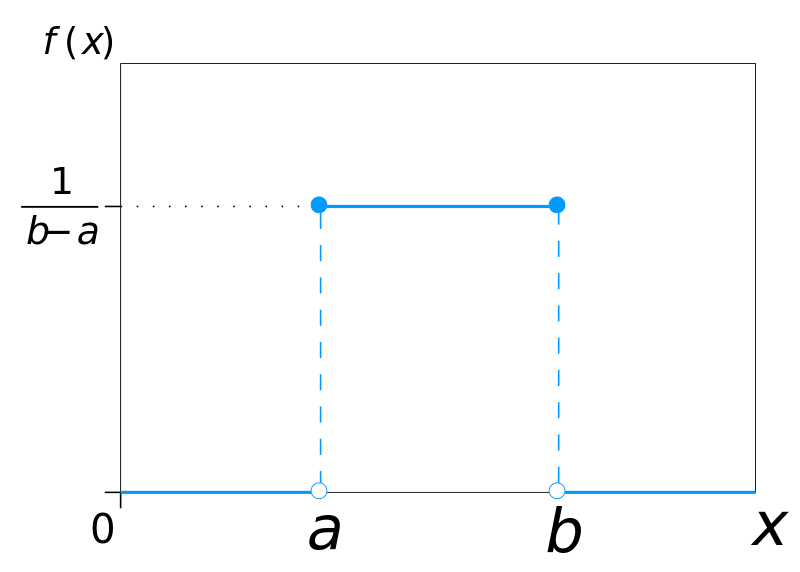
\includegraphics[width=0.5\textwidth]{figures/uniform_1.png}
  \caption{Συνάρτηση πυκνότητας πιθανότητας ομοιόμορφης κατανομής}
\end{figure}

\begin{figure}[H]
  \centering
  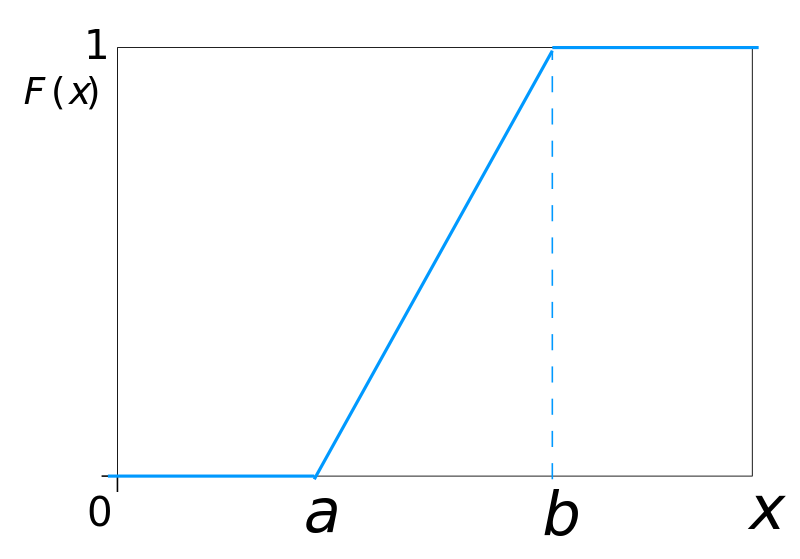
\includegraphics[width=0.5\textwidth]{figures/uniform_2.png}
  \caption{Συνάρτηση κατανομής ομοιόμορφης κατανομής}
\end{figure}

\subsubsection{Κανονική Κατανομή}

Η κανονική κατανομή, γνωστή και ως κατανομή Gauss, αναφέρεται σε τυχαίες μεταβλητές με συνεχή συνάρτηση πυκνότητας πιθανότητας. Χρησιμοποιείται ως μία πρώτη προσέγγιση 
για να περιγραφούν τυχαίες μεταβλητές πραγματικών τιμών, οι οποίες τείνουν να συγκεντρώνονται γύρω από μια μέση τιμή. Η γραφική παράσταση της σχετιζόμενης συνάρτησης 
πυκνότητας πιθανότητας έχει σχήμα "καμπάνας", και είναι γνωστή ως Γκαουσιανή συνάρτηση ή κωδωνοειδής καμπύλη. Η συνάρτηση πυκνότητας πιθανότητας είναι η εξής:

\[P(x) = \frac{1}{{\sigma \sqrt {2\pi } }}e^{{{ - \left( {x - \mu } \right)^2 } \mathord{\left/ {\vphantom {{ - \left( {x - \mu } \right)^2 } {2\sigma ^2 }}} \right. \kern-\nulldelimiterspace} {2\sigma ^2 }}}\]

Η παράμετρος \(\mu\) αποτελεί τη μέση τιμή (mean) της κατανομής και η παράμετρος \(\sigma\) την τυπική απόκλιση (standard deviation) της κατανομής. 

\begin{figure}[H]
  \centering
  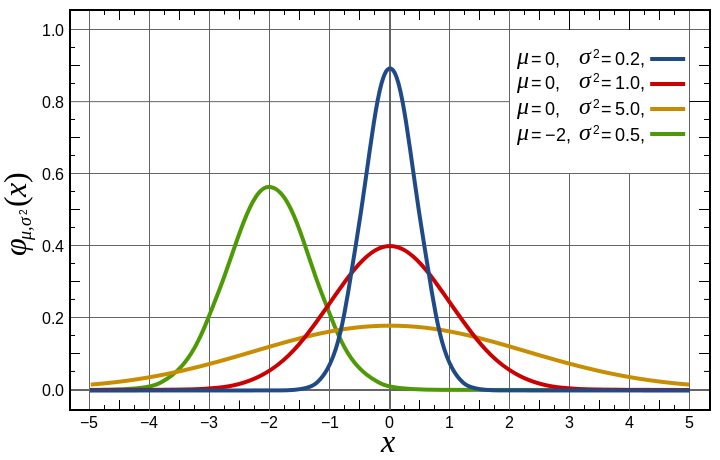
\includegraphics[width=0.5\textwidth]{figures/gauss_1.png}
  \caption{Συνάρτηση πυκνότητας πιθανότητας κανονικής κατανομής}
\end{figure}

\begin{figure}[H]
  \centering
  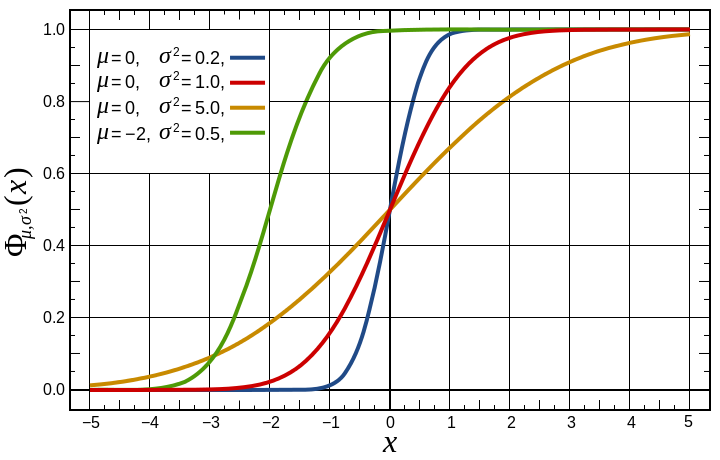
\includegraphics[width=0.5\textwidth]{figures/gauss_2.png}
  \caption{Συνάρτηση κατανομής κανονικής κατανομής}
\end{figure}

Σύμφωνα με έναν 
εμπειρικό κανόνα, στην κανονική κατανομή, οι τιμές, που είναι ανάμεσα στη μέση τιμή και μία τυπική απόκλιση μακριά, αποτελούν το 68.27\% των συνολικών τιμών, 
όσες είναι δύο τυπικές αποκλίσεις μακριά το 95.45\% και όσες είναι τρεις τυπικές αποκλίσεις μακριά το 99.73\%. 

\begin{figure}[H]
  \centering
  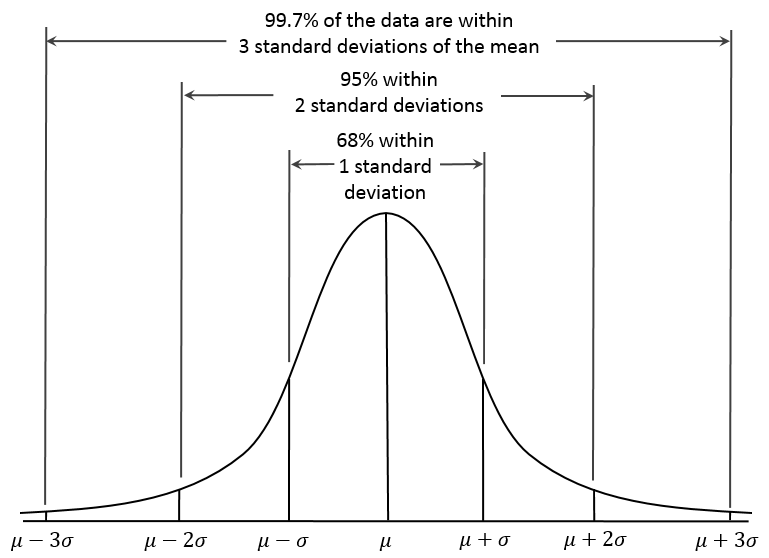
\includegraphics[width=0.6\textwidth]{figures/Empirical_Rule.PNG}
  \caption{Εμπειρικός κανόνας συσσώρευσης τιμών στην κανονική κατανομή}
\end{figure}
